\newpage
\section*{CHAPTER 4. EXPERIMENTAL RESULTS}
\phantomsection\addcontentsline{toc}{section}{CHAPTER 4. EXPERIMENTAL RESULTS}
\setcounter{section}{4}
\setcounter{subsection}{0}
\setcounter{subsubsection}{0}
\setcounter{paragraph}{0}
\setcounter{figure}{0}
\setcounter{table}{0}

Chapter 4 presents the experimental procedure and evaluation results of the proposed quantized HiFiC GAN accelerator. Following an evaluation-oriented structure, this chapter first describes the accuracy evaluation environment and the quantization results, then reports FPGA resource utilization, analyzes performance, compares the hardware-oriented implementation with the software reference, and finally summarizes the main observations.

%%%%%%%%%%%%%%%%%%%%%%%%%%%%%%%%%%%%%%%%%%%%%%%%%%%%%%%%%%%%%%%%%%%%%%%%%%%%%%%%%%%
\subsection{Accuracy Evaluation}

The first objective of the evaluation is to verify that the hardware-oriented implementation preserves the functional behavior of the HiFiC inference pipeline. Since the proposed accelerator implements the complete generator, the verification process compares the HLS/FPGA-oriented output with the Python reference model using the same input tensors and model parameters.

\subsubsection{Verification Environment}

The overall testing methodology is shown in Figure~\ref{fig:testing_env}. A set of test images ($256 \times 256$ RGB) drives two paths in parallel: the proposed HiFiC GAN accelerator running on the ZCU104 FPGA (the design under test) and a reference model, namely the original HiFiC FP32 network implemented in Python/PyTorch. For each test item, the accelerator output is compared against the reference output to produce a PASS/FAIL verdict for hardware behavior verification, while the reconstructed images are compared to quantify quality and performance through metrics such as speedup, PSNR/SSIM, latency, and compression ratio.

\begin{figure}[H]
    \centering
    
\includegraphics[width=\textwidth]{Images/testing_env.png}
    \caption{Testing environment: the accelerator under test compared against the HiFiC FP32 reference model}
    \label{fig:testing_env}
\end{figure}

Figure~\ref{fig:system_architecture} illustrates the verification and deployment environment used in this thesis. The system follows a hardware--software co-design approach on the ZCU104 platform. The Processing System (PS) is responsible for software control, memory management, and accelerator invocation, while the Programmable Logic (PL) implements the custom generator accelerator.

\begin{figure}[H]
    \centering
    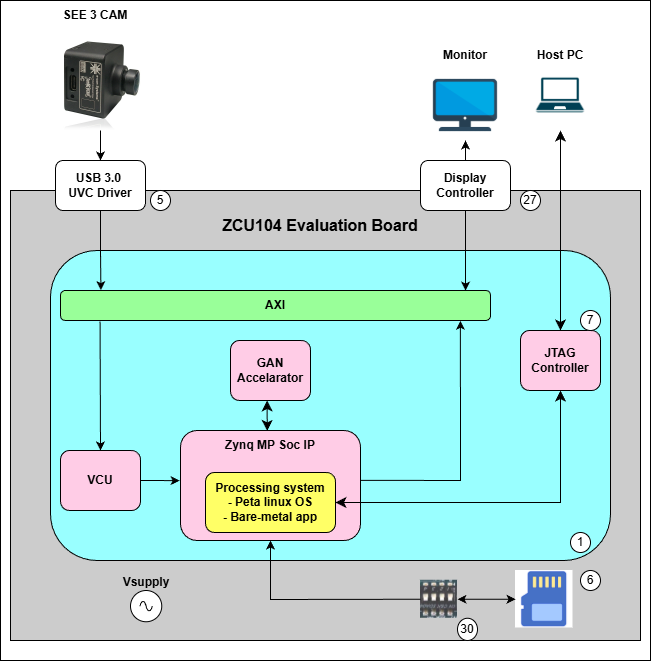
\includegraphics[width=1\linewidth]{Images/System Architecture.png}
    \caption{Verification and deployment environment on the ZCU104 platform}
    \label{fig:system_architecture}
\end{figure}

The software reference is executed in Python to generate golden outputs for comparison. The same input tensors, weights, and normalization parameters are then used by the HLS C/C++ implementation. During simulation, the output of the HLS model is compared with the Python reference to verify numerical consistency. After successful HLS verification, the generated IP core is integrated into the Vivado block design shown in Figure~\ref{fig:vivado_block_design}.

\begin{figure}[H]
    \centering
    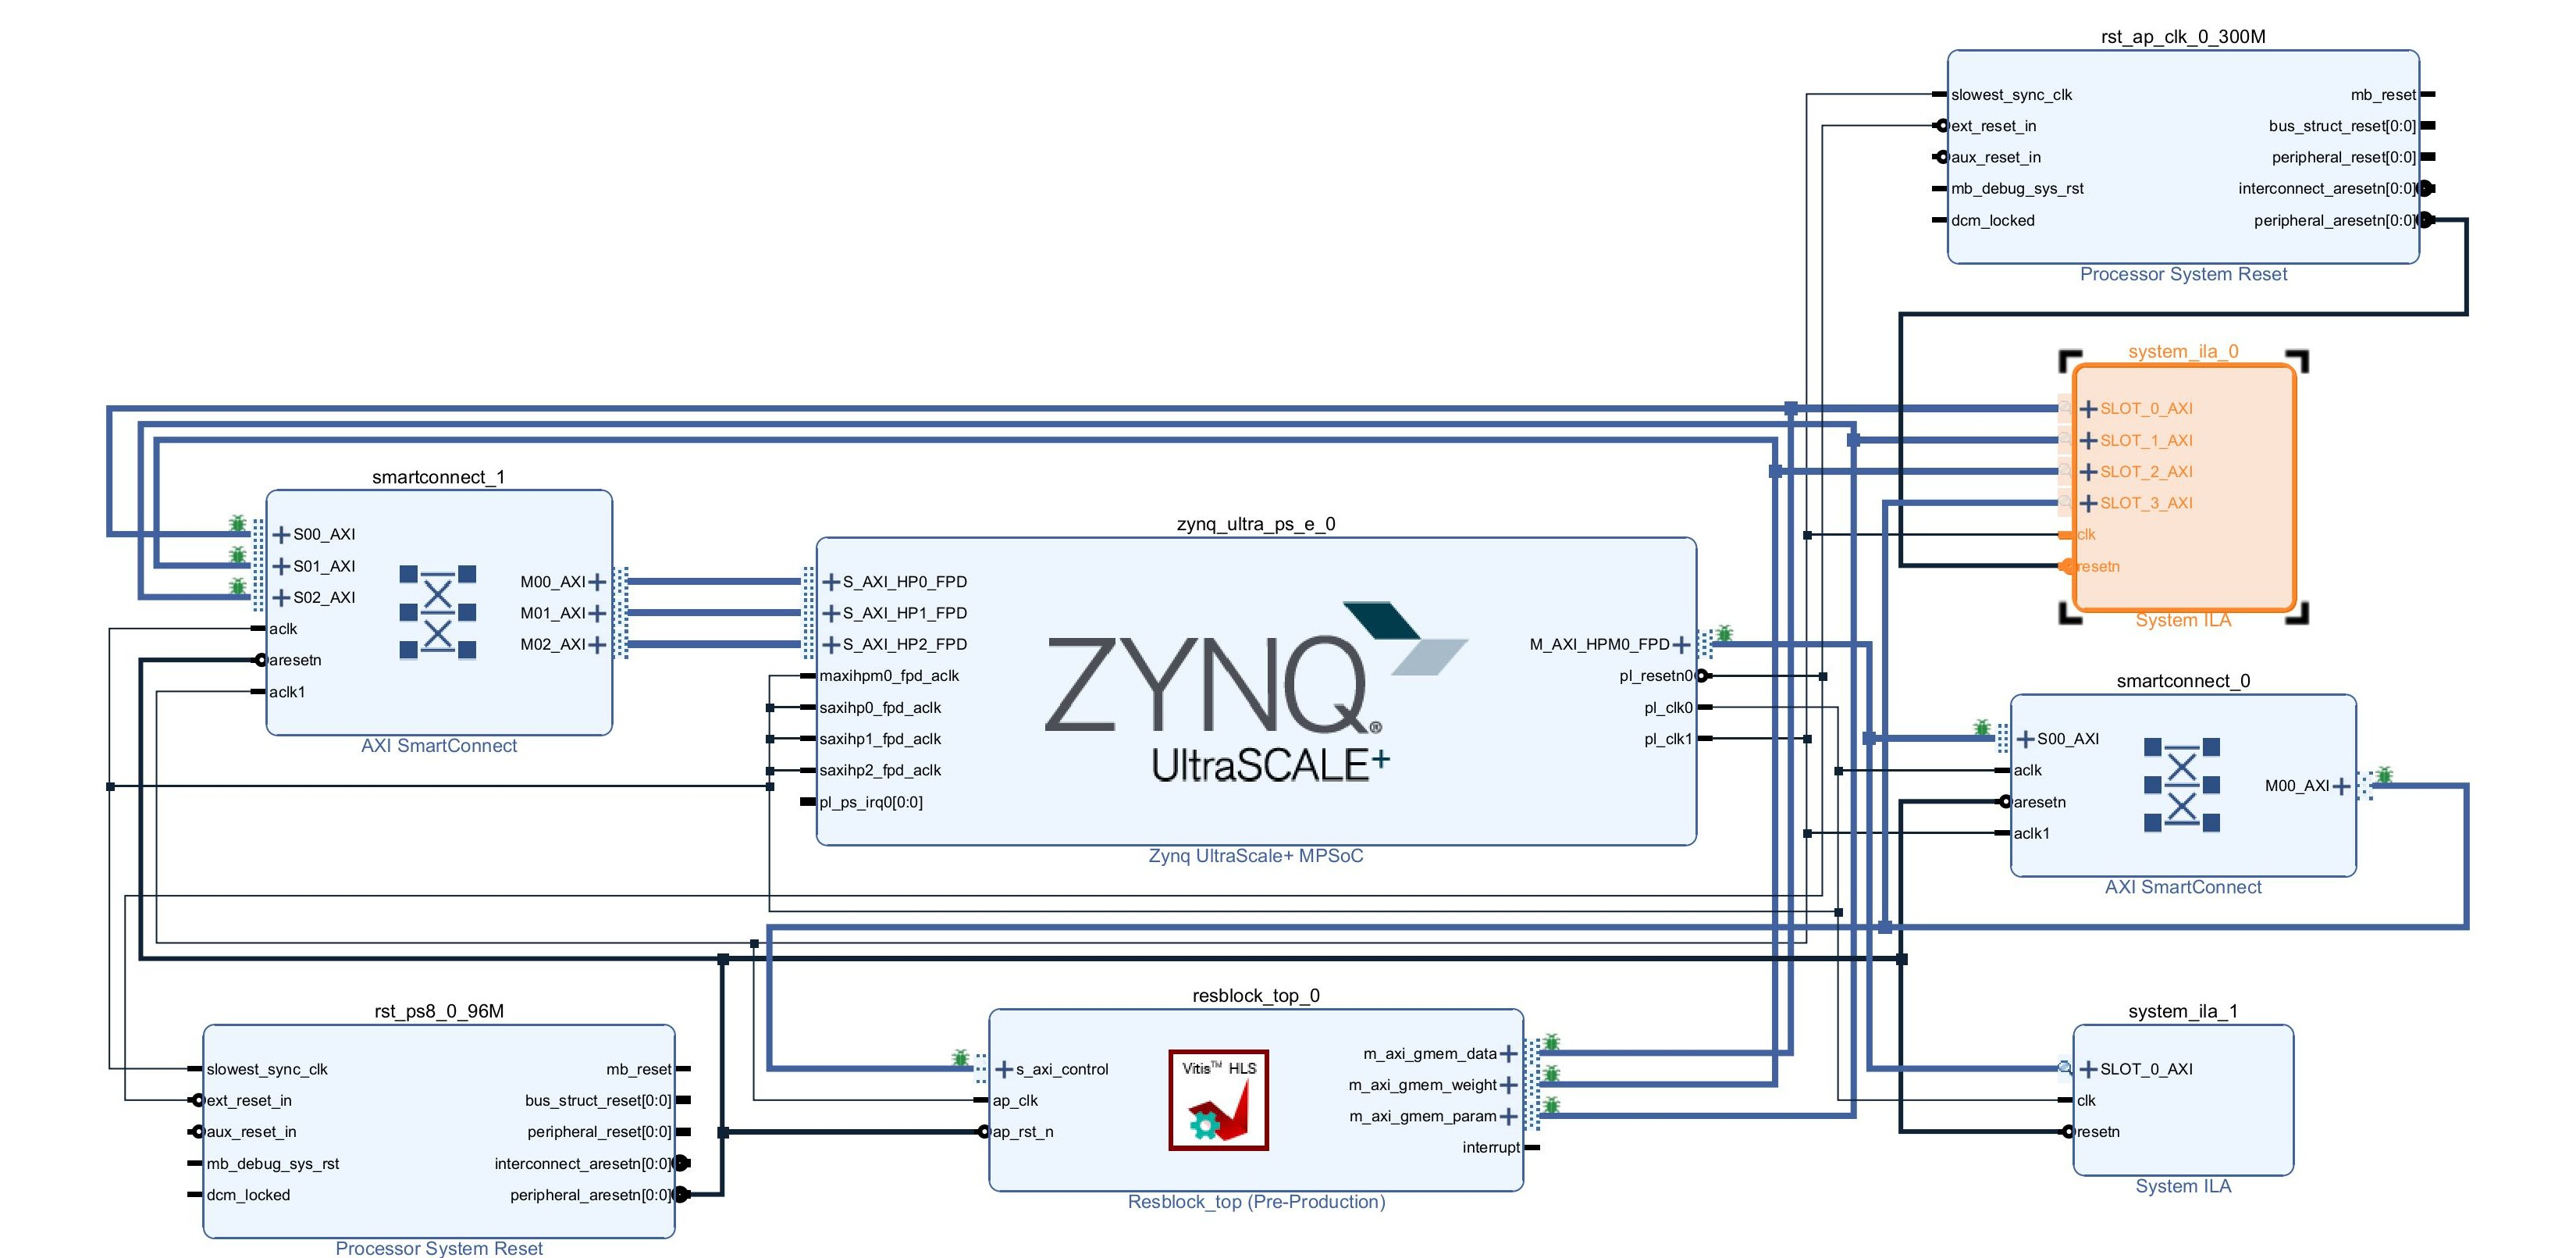
\includegraphics[width=1\linewidth]{Images/block_design.jpg}
    \caption{Vivado block design of the proposed accelerator system}
    \label{fig:vivado_block_design}
\end{figure}

The target board used for implementation is the Zynq\texttrademark{} UltraScale+\texttrademark{} MPSoC ZCU104, shown in Figure~\ref{fig:ZCU}. The most relevant components for this thesis are summarized in Table~\ref{tab:zcu104_components}. These components provide the processing system, programmable logic, external memory, SD-card boot interface, and display/output connections required for testing the accelerator.

\begin{figure}[H]
    \centering
    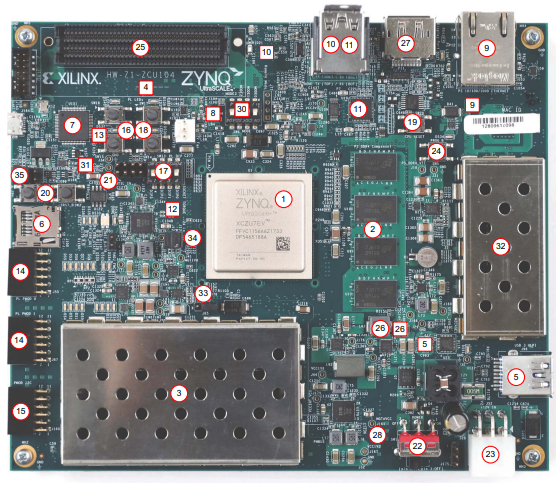
\includegraphics[width=0.9\linewidth]{Images/ZCU.png}
    \caption{Zynq\texttrademark{} UltraScale+\texttrademark{} MPSoC ZCU104 evaluation board}
    \label{fig:ZCU}
\end{figure}

\begin{table}[H]
    \centering
    \caption{Relevant ZCU104 components for accelerator evaluation}
    \label{tab:zcu104_components}
    \begin{tabular}{|c|l|}
        \hline
        \textbf{No.} & \textbf{Component} \\
        \hline
        1 & Zynq UltraScale+ XCZU7EV MPSoC \\
        \hline
        3 & PL-side SODIMM DDR4 memory \\
        \hline
        5 & USB 3.0 transceiver and USB 2.0 ULPI PHY \\
        \hline
        6 & SD-card interface connector \\
        \hline
        7 & Programmable Logic JTAG \\
        \hline
        27 & DisplayPort connector \\
        \hline
    \end{tabular}
\end{table}

The verification flow consists of four main steps. First, the Python reference model produces the expected reconstructed output or intermediate feature output. Second, the HLS C/C++ model processes the same input data using the hardware-oriented implementation. Third, the two outputs are compared using objective image-quality metrics. Finally, after synthesis and implementation, the accelerator is controlled from Vitis on the ZCU104 platform to measure board-level behavior.

\subsubsection{Test Images and Evaluation Metrics}

The evaluation uses representative RGB images resized to $256 \times 256$, consistent with the input size used throughout this thesis. The reconstructed images are evaluated using image-quality metrics introduced in Chapter~2, including Peak Signal-to-Noise Ratio (PSNR), Structural Similarity Index Measure (SSIM), and Mean Squared Error (MSE). These metrics are suitable for checking whether the quantized hardware-oriented implementation remains close to the software reference.

Figure~\ref{fig:chapter4_psnr_comparison} shows the PSNR comparison between the Python reference model and the HLS simulation model over 100 test images. The similarity of the two curves indicates that the HLS implementation follows the numerical behavior of the reference model closely enough for FPGA deployment.

\begin{figure}[H]
    \centering
    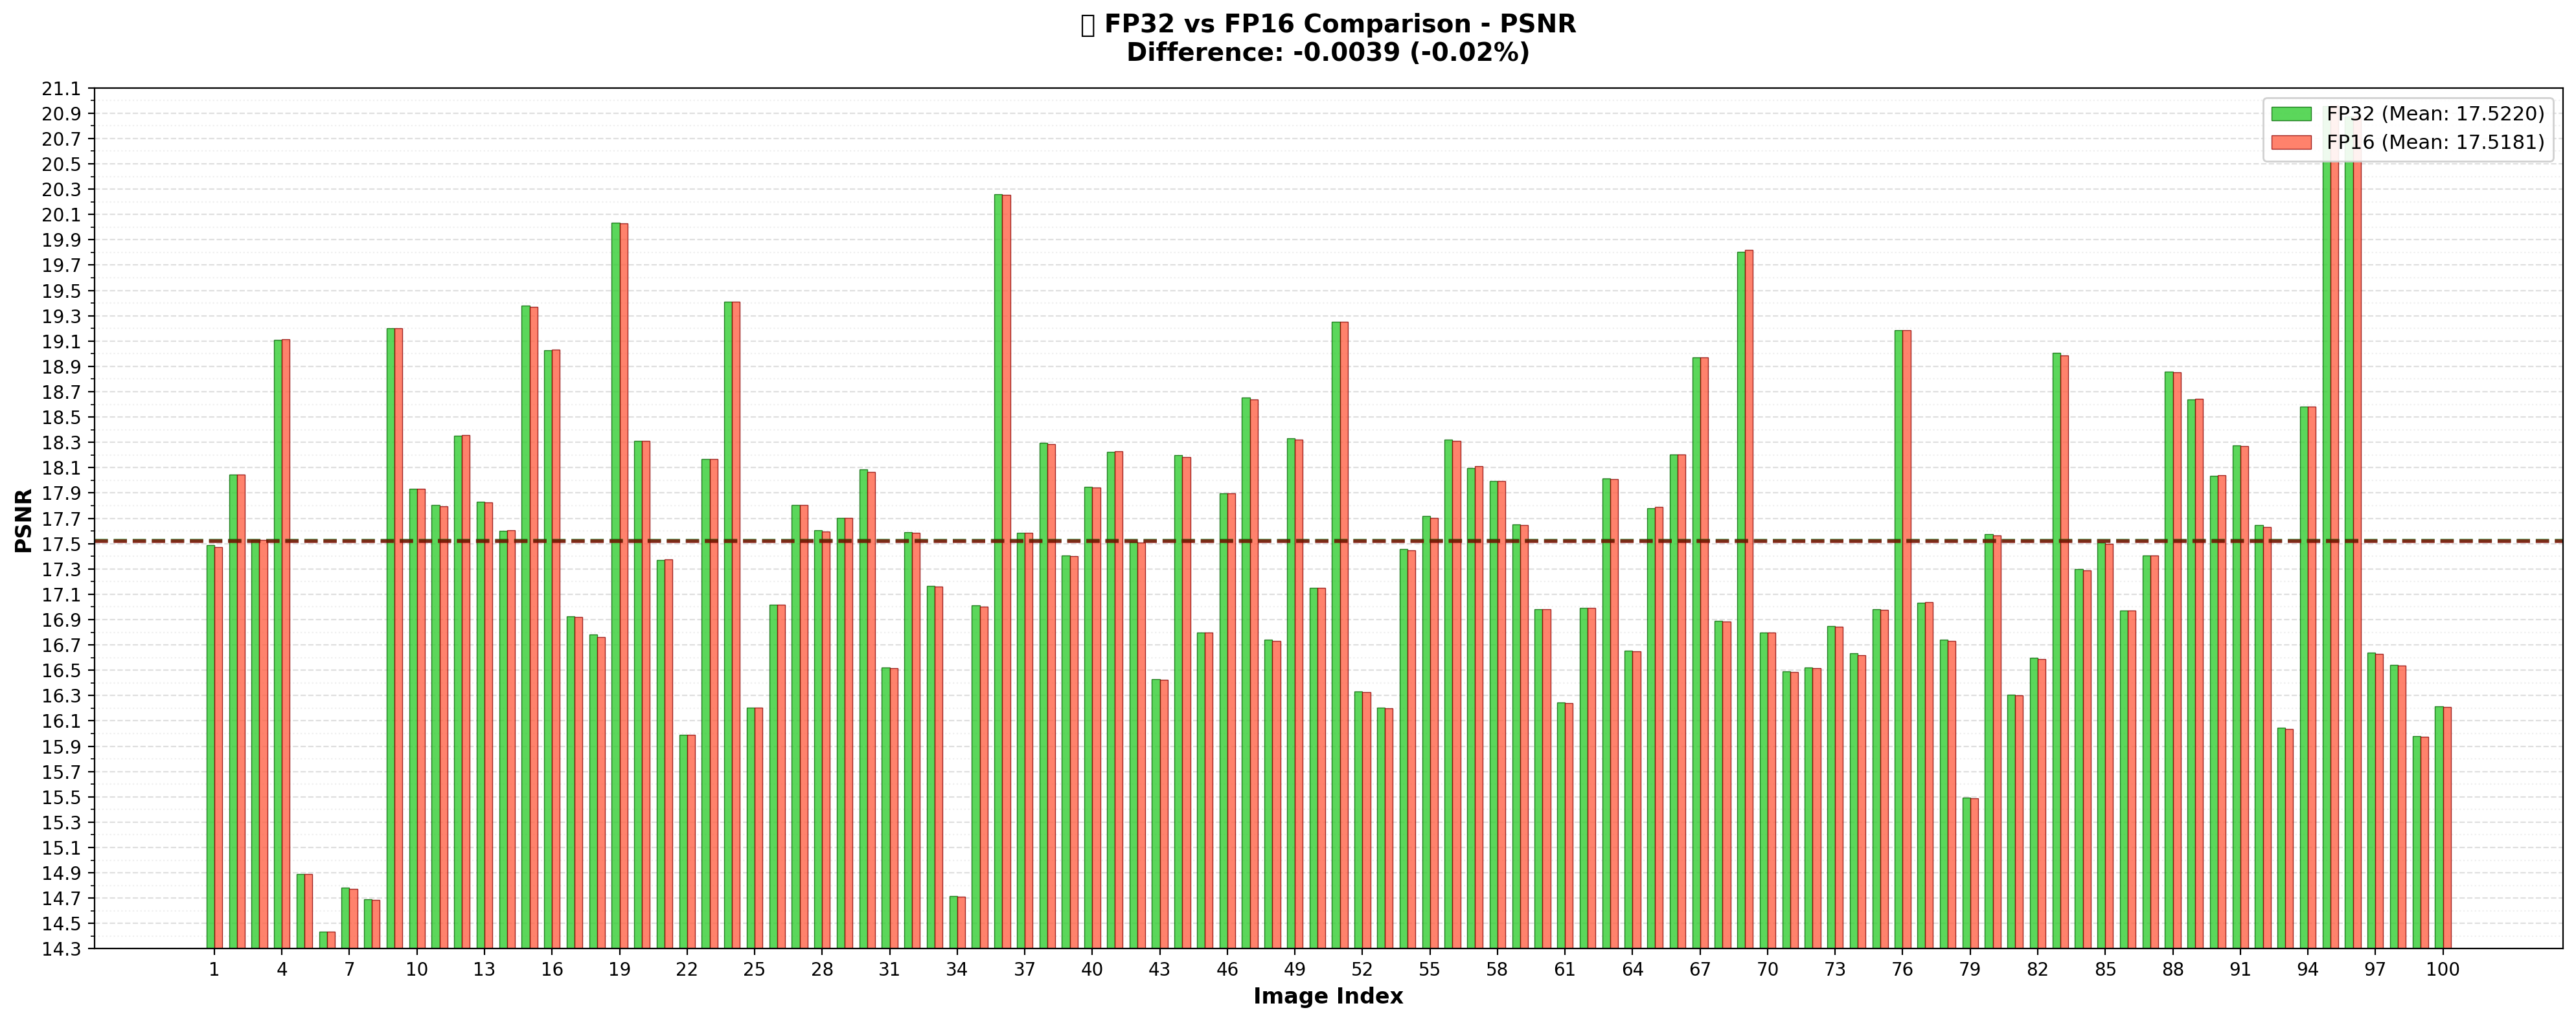
\includegraphics[width=1\linewidth]{Images/comparison_psnr_sidebyside.png}
    \caption{PSNR comparison between the Python reference model and the quantized HLS simulation model}
    \label{fig:chapter4_psnr_comparison}
\end{figure}

Overall, the accuracy evaluation confirms that the hardware-oriented ResBlock implementation preserves the main reconstruction behavior of the HiFiC generator. Small numerical differences are expected because the accelerator uses a mixed-precision data path, but the observed quality trend remains close to the Python reference.

\subsubsection{Mixed-Precision Quantization Results}

This subsection evaluates the impact of the mixed-precision quantization described in Chapter~3, i.e., the transition from full-precision FP32 computation to a mixed-precision FP16 implementation, on compression efficiency and reconstructed image quality. The experiment uses a representative test image with a resolution of $256 \times 256$. Two configurations are compared under identical conditions: the baseline FP32 model and the quantized mixed-precision FP16 model, where internal computations operate in FP16 while input and output interfaces remain in FP32. Table~\ref{tab:quant_results} summarizes the quantitative compression metrics obtained from both models.

\begin{table}[H]
\centering
\caption{Comparison between FP32 and FP16 mixed-precision HiFiC models}
\label{tab:quant_results}
\begin{tabular}{|l|c|c|c|}
\hline
\textbf{Metric} & \textbf{FP32} & \textbf{FP16 Mixed} & \textbf{Delta} \\
\hline
Original Size (bytes) & 25,879 & 25,879 & 0 \\
Bitstream Size (bytes) & 6,522 & 6,517 & -5 \\
Output Image Size (bytes) & 97,596 & 97,496 & -100 \\
Compression Ratio & 3.97$\times$ & 3.97$\times$ & 0.00 \\
Space Saving (\%) & 74.80 & 74.82 & +0.02 \\
Bits Per Pixel (bpp) & 0.7961 & 0.7955 & -0.0006 \\
PSNR (dB) & 19.08 & 19.05 & -0.03 \\
SSIM & 0.8315 & 0.8314 & -0.0001 \\
MSE  &  804.315755 & 808.560496 & 4.244 \\
\hline
\end{tabular}
\end{table}

The results indicate that the compression performance of the HiFiC model is preserved after quantization. The bitstream size is slightly reduced, while the compression ratio and space-saving metrics remain unchanged. This suggests that the probability distribution of the latent representation is not significantly affected by FP16 rounding errors, allowing the entropy coding process to operate efficiently. From a perceptual quality perspective, the degradation introduced by mixed-precision computation is negligible: the observed PSNR reduction of 0.03~dB is well below the threshold of perceptual visibility, and the SSIM metric remains nearly identical between the two configurations.

Figure~\ref{fig:quant_visual} provides a visual comparison between the reconstructed images produced by the FP32 and FP16 models. No visible artifacts or structural distortions are observed in the quantized output, confirming that the proposed mixed-precision quantization strategy achieves a favorable balance between numerical efficiency and output fidelity.

\begin{figure}[H]
    \centering
    
\includegraphics[width=0.45\linewidth]{Images/originial.png}
    \hfill
    
\includegraphics[width=0.45\linewidth]{Images/quantized picture.png}
    \caption{Visual comparison of reconstructed images: FP32 model (left) and FP16 mixed-precision model (right)}
    \label{fig:quant_visual}
\end{figure}

% =====================================================================
% NOTE (Quoc Anh review): hai waveform GAN duoi day lay tu luong synthesis
% cu cua bao cao thi. Giu lai lam minh chung verification chuc nang o muc
% tin hieu; neu da co waveform moi cua ResBlock accelerator thi thay vao.
% Neu thay khong con phu hop, co the xoa block nay.
% =====================================================================
% To verify functional correctness at the signal level, the input and output data streams of the generator block were captured as simulation waveforms. Figure~\ref{fig:gan_waveform} and Figure~\ref{fig:gan_weight_waveform} show the input and output data, respectively, confirming that the generation process produces the expected results.

% \begin{figure}[H]
%     \centering
%     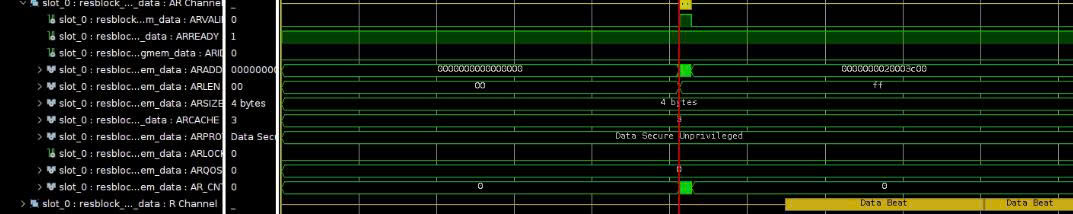
\includegraphics[width=1\linewidth]{Images/waveform.jpg}
%     \caption{Input data waveform of the generator block}
%     \label{fig:gan_waveform}
% \end{figure}
% \begin{figure}[H]
%     \centering
%     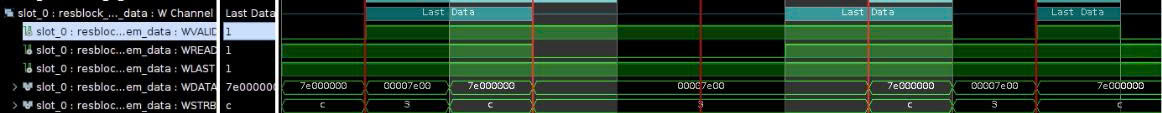
\includegraphics[width=1\linewidth]{Images/wave_w.jpg}
%     \caption{Output data waveform of the generator block}
%     \label{fig:gan_weight_waveform}
% \end{figure}

%%%%%%%%%%%%%%%%%%%%%%%%%%%%%%%%%%%%%%%%%%%%%%%%%%%%%%%%%%%%%%%%%%%%%%%%%%%%%%%%%%%
\subsection{Resource Utilization and Power Measurement}

After functional verification, the complete generator accelerator was synthesized and implemented on the ZCU104 FPGA platform to evaluate resource utilization. The implementation result reflects the cost of mapping all three generator stages (Fusion, UpConv, and Conv77), their local buffering, AXI-based data movement, and control logic into the Programmable Logic (PL). The target clock frequency is 300~MHz, and the implemented design closes timing with a maximum frequency of 308.74~MHz.

The hardware utilization report is summarized in Table~\ref{tab:hific_generator_utilization}. The implemented accelerator uses 205,233 LUTs, corresponding to 89\% of the available LUT resources, and approximately 189,763 FFs, corresponding to 41\% of the available flip-flop resources. For on-chip storage, the design consumes 510 BRAM 18Kb blocks, or 82\% of the available BRAM resources, together with all 96 URAM blocks (100\%). The arithmetic datapath uses 1,550 DSP slices, corresponding to 90\% of the available DSP resources.

\begin{table}[H]
    \centering
    \caption{Hardware resource utilization of the full HiFiC generator accelerator on the ZCU104}
    \label{tab:hific_generator_utilization}
    \begin{tabular}{|l|c|}
        \hline
        \textbf{Resource} & \textbf{Full Generator Accelerator} \\
        \hline
        LUTs & 205,233 (89\%) \\
        \hline
        FFs & 189,763 (41\%) \\
        \hline
        BRAMs (18Kb Block) & 510 (82\%) \\
        \hline
        URAMs & 96 (100\%) \\
        \hline
        DSPs & 1,550 (90\%) \\
        \hline
        Max frequency (MHz) & 308.74 \\
        \hline
    \end{tabular}
\end{table}

The utilization results show that the proposed accelerator is both computation-intensive and memory-intensive. DSP utilization is high because convolution dominates the generator workload and requires a large number of multiply--accumulate operations. BRAM and URAM utilization are also high because intermediate feature maps, line buffers, weights, the up-convolution row accumulator, and the skip-connection buffers must be stored locally to reduce external DDR access and sustain the pipelined datapath; in particular, all available URAM blocks are used.

Power measurement is evaluated as part of board-level deployment. In this design, the main contributors to dynamic power are expected to be DSP activity, BRAM/URAM access, AXI memory transfers, and clocked control logic. Therefore, reducing unnecessary memory movement and improving data reuse are important not only for performance but also for power efficiency.

%%%%%%%%%%%%%%%%%%%%%%%%%%%%%%%%%%%%%%%%%%%%%%%%%%%%%%%%%%%%%%%%%%%%%%%%%%%%%%%%%%%
\subsection{Performance Evaluation}

In addition to resource utilization, several performance metrics are used to evaluate the effectiveness of the proposed accelerator. These metrics include operating frequency, throughput, accelerated block, numerical precision, and speedup compared with the software-only baseline.

Table~\ref{tab:performance_evaluation} summarizes the main performance results. The accelerator operates at 300~MHz and implements the complete HiFiC generator. The total compute volume of the generator is 90.34~GOP (counting the operations actually executed by the MAC engines), and the design processes one $256\times256$ image in 735.6~ms, giving a sustained throughput of 122.8~GOPS. The latency is dominated by the Fusion Core (568.8~ms), followed by the UpConv Core (149.0~ms) and the Conv77 Core (17.75~ms).

\begin{table}[H]
    \centering
    \caption{Performance evaluation of the proposed accelerator}
    \label{tab:performance_evaluation}
    \begin{tabular}{|l|c|}
        \hline
        \textbf{Metric} & \textbf{Result} \\
        \hline
        FPGA platform & ZCU104 (XCZU7EV) \\
        \hline
        Operating frequency & 300~MHz (Fmax 308.74~MHz) \\
        \hline
        Accelerated network & Full HiFiC generator \\
        \hline
        Precision & Mixed FP16 \\
        \hline
        Compute volume & 90.34~GOP \\
        \hline
        Total latency (per image) & 735.6~ms \\
        \hline
        Throughput & 122.8~GOPS \\
        \hline
    \end{tabular}
\end{table}

The performance result shows that the accelerator benefits from parallel DSP computation and local on-chip buffering. The Fusion Core, which executes the convolution-heavy residual blocks, reaches about 92\% of its peak MAC throughput thanks to the rotating accumulator and the overlapped convolution and normalization passes; the UpConv and Conv77 cores are less MAC-bound because their latency also includes pipeline fill/drain and boundary handling. The high BRAM, URAM, and DSP utilization indicates that further performance scaling must be balanced carefully against the remaining device resources.

%%%%%%%%%%%%%%%%%%%%%%%%%%%%%%%%%%%%%%%%%%%%%%%%%%%%%%%%%%%%%%%%%%%%%%%%%%%%%%%%%%%
\subsection{Comparison}

To the best of our knowledge, the HiFiC model has not previously been implemented on an FPGA, so there is no prior hardware accelerator of the same model to compare against directly. Therefore, this section evaluates the proposed accelerator by comparing its performance against the software execution baseline, focusing on the acceleration ratio (speedup) and throughput.

The software baseline corresponds to the full generator inference profiled on an Intel Core i9 CPU operating at 2.2~GHz, which takes 1073.19~s per image, as reported in the runtime breakdown of Table~\ref{tab:runtime_breakdown} in Chapter~3. This long CPU runtime is a direct consequence of the very large feature tensors of the generator (for example, $16\times16\times960$ inside each residual block). The proposed accelerator executes the same generator on the ZCU104 platform at 300~MHz in 735.6~ms using mixed FP16 precision. Table~\ref{tab:performance_comparison} summarizes the comparison.

\begin{table}[H]
    \centering
    \caption{Performance comparison between the software baseline and the proposed FPGA accelerator}
    \label{tab:performance_comparison}
    \begin{tabular}{|p{2.6cm}|p{3.6cm}|c|c|c|}
        \hline
        \textbf{Platform} & \textbf{Device} & \textbf{Precision} & \textbf{Latency} & \textbf{Speedup} \\
        \hline
        Software (CPU) & Intel Core i9 @ 2.2~GHz & FP32 & 1073.19~s & $1\times$ \\
        \hline
        % TODO (Quoc Anh): neu co do them tren GPU, them mot hang o day:
        % GPU & <ten GPU> & FP32/FP16 & <latency> & <speedup> \\
        Proposed FPGA & ZCU104 (XCZU7EV) @ 300~MHz & Mixed FP16 & 735.6~ms & $\approx 1459\times$ \\
        \hline
    \end{tabular}
\end{table}

The comparison shows that running the full generator on the FPGA reduces the per-image processing time from 1073.19~s on the CPU to 735.6~ms, an acceleration of approximately $1459\times$, while sustaining a throughput of 122.8~GOPS. This large speedup is obtained even though the FPGA operates at a much lower clock frequency than the CPU, because the accelerator exploits spatial parallelism through many processing elements, local on-chip buffering, and overlapped convolution and normalization passes that keep the MAC datapath busy. The result confirms that dedicated hardware is essential for the compute-bound HiFiC generator, whose very large feature tensors make plain CPU execution impractical.

% =====================================================================
% NOTE (Quoc Anh): bang so sanh hien co CPU (1073.19 s, da do thuc) vs
% FPGA (735.6 ms). Neu sau nay co them so lieu do tren GPU thi dien vao
% hang GPU (comment o bang tren) de co day du CPU / GPU / FPGA.
% =====================================================================

%%%%%%%%%%%%%%%%%%%%%%%%%%%%%%%%%%%%%%%%%%%%%%%%%%%%%%%%%%%%%%%%%%%%%%%%%%%%%%%%%%%
\subsection{Chapter Conclusion}

Chapter 4 presented the experimental results of the proposed quantized HiFiC GAN accelerator. The accuracy evaluation compared the HLS simulation output with the Python reference model using PSNR over 100 test images, and the mixed-precision quantization results showed that compression ratio, PSNR, and SSIM are preserved when moving from FP32 to FP16. The resource utilization report showed that the design uses a large portion of the available DSP, BRAM, and URAM resources (all URAM blocks are used), which is expected for a highly parallel full-generator accelerator. The performance evaluation demonstrated an operating frequency of 300~MHz (timing closed at 308.74~MHz), a total latency of 735.6~ms per image, a throughput of 122.8~GOPS, and an acceleration of approximately $1459\times$ over the CPU software baseline.

Overall, the results confirm that the proposed hardware--software co-design is suitable for accelerating the complete HiFiC generator while preserving reconstruction quality.
